% ------------------------------------------------------------------------
% ------------------------------------------------------------------------
% abnTeX2: Modelo de Artigo Acadêmico em conformidade com
% ABNT NBR 6022:2018: Informação e documentação - Artigo em publicação 
% periódica científica - Apresentação
% Atualizedo para as citações - (SILVA, 2023) para (Silva, 2023)  de acordo com a NBR 10520/2023 
% ------------------------------------------------------------------------



\documentclass[a4paper, portugues,11pt]{article}
\usepackage[brazilian]{babel}

\usepackage[utf8]{inputenc}
\usepackage[scaled]{berasans} %https://tug.org/FontCatalogue/berasans/
\renewcommand*\familydefault{\sfdefault}  %% Não encontrei a spranq eco sans para Latex, a Bera Sans é igual mas sem os furinhos
\usepackage[T1]{fontenc}
%\usepackage[latin1]{inputenc}

\usepackage{lipsum} % texto aleatório em latim

\usepackage{url}
\usepackage{setspace}

\usepackage{enumerate} % para os dois tipos de listas

\usepackage{multicol}
%\usepackage{isolatin1}
%\usepackage[dvips]{graphicx}

\usepackage[pdftex]{graphicx}
\usepackage[pdftex]{hyperref}
\usepackage[pdftex]{color}
\usepackage[pdftex]{hyperref}

\usepackage[dvipsnames]{xcolor}
%\usepackage{color}

\usepackage{pifont} %símbolos marcadores
\usepackage[normalem]{ulem} %sublinhados
%simbolos marcadores
\usepackage{amssymb}
\usepackage{indentfirst}
\usepackage{setspace}


\usepackage[
    bottom=2cm,
    top=1cm,
    left=2.5cm,
    right=1.5cm, 
    headsep=1.5cm,
    %headheight=14.5pt, %%% 3mm is too small
    %heightrounded
    includehead, 
    includefoot
    ]{geometry}


% \hyphenation{se-ma-na}

\onehalfspacing
%\singlespace

%------------------------------------------------------------------------


	
% Seleciona o idioma do documento (conforme pacotes do babel)
%\selectlanguage{english}

% ---
% PACOTES
% ---



% ---       
% Pacotes fundamentais 
% ---
%\usepackage{lmodern}			% Usa a fonte Latin Modern
%\usepackage{mathptmx} % Fonte times new romam no texto
%\usepackage{ccfonts}

\usepackage{nomencl} 			% Lista de simbolos
\usepackage{color}				% Controle das cores
\usepackage{graphicx}			% Inclusão de gráficos
\usepackage{microtype} 			% para melhorias de justificação
% ---
		
% ---
% Pacotes adicionais, usados apenas no âmbito do Modelo Canônico do abnteX2
% ---
\usepackage{lipsum}				% para geração de dummy text
% ---
		
% ---
% Pacotes de citações
% ---

\usepackage[alf]{abntex2cite}	% Citações padrão ABNT
% ---







% alterando o aspecto da cor azul
\definecolor{blue}{RGB}{41,5,195}

\makeatother
% --- 


%\usepackage{fancyhdr} %cabeçalhos
\usepackage{fancyhdr,xpatch}
\fancyhf{} % limpa os cabeçalho e rodapés
\pagestyle{fancy} % sem definir esse comando, o cabeçalho personalizado não é exibido

\fancyhead{} % define o cabeçalho personalizado
\renewcommand{\headrulewidth}{0.1mm}
\lhead{
\includegraphics[angle=0, width=0.15\textwidth]{Imagens/logo-serpro.jpg}}
\chead{}
\rhead{\large \textbf{1º Prêmio Serpro de Inovação}}

\fancyfoot{}
\renewcommand{\footrulewidth}{0.1mm}
\lfoot{\footnotesize SGAN Av.L-2 Norte Quadra 601 - Módulo G  \\ Asa Norte, Brasília - DF - CEP: 70830-900}
\cfoot{}
\rfoot{\footnotesize
{\sf \textbf{\color{gray}\large www.serpro.gov.br}} \\
\vspace*{5mm}
\thepage
}



% ----
% Configurar primeiras seções e sumário

\makeatletter
\let\ORI@section\section
\renewcommand{\section}{\@ifstar\s@section\ORI@section}
\newcommand{\s@section}[1]{%
  \ORI@section*{#1}
  \csname phantomsection\endcsname % for hyperref
  \addcontentsline{toc}{section}{#1}
}
\xpatchcmd{\tableofcontents}{\section}{\ORI@section}{}{} % toc not in toc
\makeatother

% ----



\begin{document}

\newgeometry{top=20mm, bottom=20mm, right=20mm, left=20mm}
\thispagestyle{empty}

\begin{figure}[!htbp]
  \begin{center}
    
\includegraphics[angle=0, width=0.91\textwidth]{Imagens/capa-ps.jpg}
  \end{center}
 \end{figure}

 \begin{center}
  {\huge \{Título do Trabalho\}}

	%\textbf{\LARGE Modelo em \LaTeX para o Prêmio Serpro}
\end{center}

\restoregeometry % 
\clearpage

\pagenumbering{roman}

\tableofcontents
\clearpage

\listoffigures
\clearpage

\listoftables 
\clearpage

\section*{Section A}

\clearpage
\pagenumbering{arabic}


% Retira espaço extra obsoleto entre as frases.
\frenchspacing 



%\maketitle
% ----------------------------------------------------------
% ELEMENTOS TEXTUAIS
% ----------------------------------------------------------

% \textual


% ----------------------------------------------------------
% Introdução
% ----------------------------------------------------------

%\setcounter{section}{3}
\section{Título do Pré-projeto de Pesquisa}
\section{Tema do trabalho de conclusão de curso}

(O que vai ser pesquisado)
Explicar brevemente o assunto que deseja desenvolver.
Elaborar uma apresentação sucinta do assunto que será abordado na pesquisa.
Apresentar genericamente o tema, anunciar a ideia básica do que se deseja pesquisar, situar o tema dentro do contexto geral do seu
campo de atuação profissional, descrever as movações que levaram à escolha do tema e indicar o objeto de análise, jusficando a originalidade
da abordagem.

Minha pesquisa no mestrado na UFRN e na RNP foi focada em protocolos de rede e roteamento IP Multicast \cite{weldsonufrn}. Nos anos seguintes os resultados da pesquisa foram aplicados em atividades de ensino, docência e publicados em periódicos internacionais relevantes \cite{weldson2004} \cite{DBLP:conf/policy/FrancoLSPATGBJF06} \cite{DBLP:conf/noms/LimaAVATG06}. A partir de 2005 meus estudos passaram a assumir um caráter menos acadêmico e mais profissional, realizei inúmeros treinamentos e capacitações técnicas em tecnologia e desenvolvi pesquisa aplicada a grandes redes públicas. Em função da pesquisa aplicada recebi diversas premiações internas no Serviço Federal de Processamento de Dados (SERPRO), onde passei a trabalhar desde 2005.

\section{Problema}

(Qual a pergunta a ser respondida por esta pesquisa?)
Informar o problema central da pesquisa.
Pode ser apresentado de forma destacada no texto, em um tópico específico, ou estar inserido no corpo do texto, desde que seja de
fácil idenficação ao leitor/examinador.
Colocar o problema de pesquisa em formato de pergunta, quesonando uma dada realidade.
Dar preferência às questões prácas que envolvem a área de atuação profissional do candidato. Figura \ref{fig:soap} apresenta o esqueleto de uma mensagem SOAP. O \texttt{soap:Envelope} é o elemento raiz do documento XML.

\begin{figure}[!htbp]
 \begin{center}
 \begin{tabular}[htb]{|c|}
 \hline
 \begin{minipage}[b]{0.8\linewidth}
 \vspace*{2mm}
 \texttt{\footnotesize
{\color{Gray}\footnotesize \ 01. }<?xml version="1.0"?> \\
{\color{Gray}\footnotesize \ 02. }<soap:Envelope \\
{\color{Gray}\footnotesize \ 03. }xmlns:soap=``http://www.w3.org/2001/12/soap-envelope'' \\
{\color{Gray}\footnotesize \ 04. }soap:encodingStyle=``http://www.w3.org/2001/12/soap-encoding''> \\
{\color{Gray}\footnotesize \ 05. }\hspace{5mm}<soap:Header> \\
{\color{Gray}\footnotesize \ 06. }\hspace{10mm}... \\
{\color{Gray}\footnotesize \ 07. }\hspace{5mm}</soap:Body> \\
{\color{Gray}\footnotesize \ 08. }</soap:Envelope> \\
   }
 \end{minipage}
 \\ \hline
 \end{tabular}
 \caption{Exemplo de mensagem SOAP} \label{fig:soap}
 \end{center}
\end{figure}

\section{Justificativa do Estudo}

(Qual a importância de se pesquisar este tema?)
Apresentar, de forma clara e objeva, as razões de ordem teórica ou práca que jusficam a realização da pesquisa, enfazando o
caráter de originalidade do estudo.

\begin{itemize}
  \item[\ding{51}] Code 51
  \item[\ding{52}] Code 52
  \item[\ding{54}] Code 54
  \item[\ding{55}] Code 55
  \item[\ding{212}] Code 212
  \item default
\end{itemize}

Mostrar a relevância do problema a ser invesgado e as contribuições que a pesquisa pode trazer, no sendo de proporcionar
respostas aos problemas propostos ou a possibilidade de sugerir modificações no âmbito da realidade retratada pelo tema.
Indicar a importância da pesquisa sobre a temáca escolhida para a instuição de trabalho do candidato.


\begin{enumerate}
  \item One
  \item Two
  \item Three
\end{enumerate}

\section{Metodologia}

(Como a pesquisa será realizada?)
Mostrar como será desenvolvida a pesquisa para agir os objevos propostos.
Deve descrever sucintamente o po de pesquisa a ser abordada (bibliográfica, documental, exploratória, de campo, estudo de caso,
etc.).
Delimitar o tempo e o espaço que serão empregados na pesquisa, bem como a fonte dos dados que serão coletados e os
instrumentos escolhidos para a coleta (entrevistas, formulários, quesonários, legislação, banco de dados, etc.).


\begin{table}[htb]
  \begin{center}
  \begin{tabular}{|l|l||c|c|c|c|c|c|c|}
  \hline
  \multicolumn{2}{|c|}{\bf Dia} & \multicolumn{2}{|c|}{\bf Manhã} & \multicolumn{2}{|c|}{\bf Tarde} & \multicolumn{2}{|c|}{\bf Noite} & {\bf Total} \\ \cline{3-9}
  \multicolumn{2}{|c|}{\bf }  & {\bf \ E \ } & {\bf \ S \ } & {\bf  \ E \ } & {\bf \ S \ } & {\bf \ E \ } & {\bf \ S \ } & {\bf hs} \\
      \hline \cline{1-09}
  
  {\bf 01} & {\bf Domingo} & \colorbox{Gray}{\hspace{6mm}} & \colorbox{Gray}{\hspace{6mm}} & \colorbox{Gray}{\hspace{6mm}} & \colorbox{Blue}{\hspace{6mm}} & \colorbox{Gray}{\hspace{6mm}} & \colorbox{Gray}{\hspace{6mm}} & \colorbox{Gray}{\hspace{9mm}}  \\ \hline 
  {\bf 02} & {\bf Segunda} &  &  &  &  & - & - &   \\ \hline
  {\bf 03} & {\bf Terça} &  &  &  &  &  - & - &  \\ \hline 
  {\bf 04} & {\bf Quarta} &  &  &  &  &  - & - &  \\ \hline  
  {\bf 05} & {\bf Quinta} &  &  &  &  &  - & - &  \\ \hline
  {\bf 06} & {\bf Sexta} &  &  &  &  &  - & - &  \\ \hline
  {\bf 07} & {\bf Sábado} & \colorbox{Gray}{\hspace{6mm}} & \colorbox{Gray}{\hspace{6mm}} & \colorbox{Gray}{\hspace{6mm}} & \colorbox{Gray}{\hspace{6mm}} & \colorbox{Gray}{\hspace{6mm}} & \colorbox{Gray}{\hspace{6mm}} & \colorbox{Gray}{\hspace{9mm}}  \\ \hline 
  {\bf 08} & {\bf Domingo} & \colorbox{Gray}{\hspace{6mm}} & \colorbox{Gray}{\hspace{6mm}} & \colorbox{Gray}{\hspace{6mm}} & \colorbox{Gray}{\hspace{6mm}} & \colorbox{Gray}{\hspace{6mm}} & \colorbox{Gray}{\hspace{6mm}} & \colorbox{Gray}{\hspace{9mm}}  \\ \hline 
  {\bf 09} & {\bf Segunda} &  &  &  &  &  18:00 & 22:00 &  4:00 \\ \hline \cline{1-09}
  % {\bf 15} & {\bf Terça} & X & X & X & X & X & X & FERIADO & X \\ \hline 
  % {\bf 29} & {\bf Sábado} &  &  &  &  \colorbox{Gray}{\hspace{6mm}}  &  &  &  &  \\ \hline \cline{1-10}
  \multicolumn{8}{|r|}{\bf Total de horas presenciais no mês \ \ } & 64:00 \\ \hline
  \end{tabular}
  \caption{Tabela complexa} \label{tab:comp}
  \end{center}
  \end{table}


\section{Objetivos e resultados Esperados} \label{sec:obj}
(O que se quer idenficar na pesquisa?)
Descrever o objevo principal da pesquisa que irá desenvolver.
Expressar em uma sentença curta e de fácil entendimento o que o pesquisador pretende angir com sua invesgação. (ex. um
diagnósco, uma avaliação de políca ou Programa de Governo, uma proposta de intervenção na realidade).
Evidenciar a contribuição para o campo profissional do candidato.

Com  a conclusão de meu MBA na ENAP em 2024.

\begin{multicols}{2}
  \lipsum[10]
\end{multicols}


\begin{figure}[!htbp]
  \begin{center}
    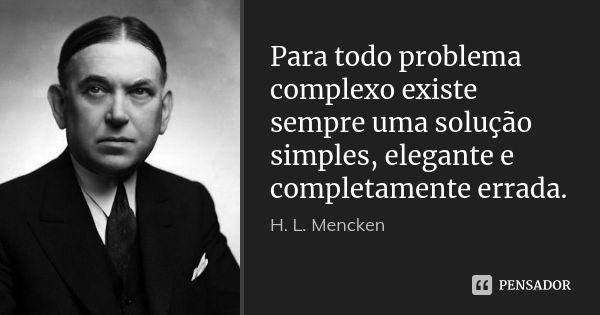
\includegraphics[angle=0, width=0.7\textwidth]{Imagens/h_l_mencken.jpg}
  \caption{{\bf Prejudices: Second Series} - Página 158, de Henry Louis Mencken - Publicado por Alfred A. Knopf, 1920 - 254 páginas} \label{fig:rg}
  \end{center}
 \end{figure}

\lipsum[3]


% ----------------------------------------------------------
% Referências bibliográficas
% ----------------------------------------------------------
\bibliographystyle{tex/abntex2-alf.bst}
\bibliography{abntex2-references}

% ----------------------------------------------------------
% Glossário
% ----------------------------------------------------------
%
% Há diversas soluções prontas para glossário em LaTeX. 
% Consulte o manual do abnTeX2 para obter sugestões.
%
%\glossary

% ----------------------------------------------------------
% Apêndices
% ----------------------------------------------------------

% ---
% Inicia os apêndices
% ---

% ---

% ----------------------------------------------------------
% Anexos
% ----------------------------------------------------------

% ----------------------------------------------------------
% Agradecimentos
% ----------------------------------------------------------



\end{document}
